\documentclass[11pt,ngerman]{scrartcl}

% standard packages
\usepackage[utf8]{inputenc}  % input in UTF-8
\usepackage[T1]{fontenc}  % output in T1 fonts (westeuropäische Codierung)
\usepackage{lmodern}  % latin modern fonts
\usepackage[ngerman]{babel}  % deutsches Sprachpaket, neue Rechtschreibung

% Seitensetup
\usepackage{scrlayer-scrpage}  % Seitenformatierung durch KOMA-interne Optionen
\usepackage[top=4cm, bottom=4cm]{geometry}  % Seitengeometrie (kann durch KOMA ersetzt werden, hab ich aber nicht geschafft)
\usepackage[hypcap=false]{caption, subcaption}  % caption editing - hypcap warning with hyperref
\usepackage{array}  % table editing

% additional packages
\usepackage{amsmath, amssymb, amstext}  % math packages (American Math Society)
\usepackage{bm}
\usepackage{icomma}  % Kommata in Dezimalzahlen verursachen keinen Abstand mehr
\usepackage{graphicx}  % Bilder einfügen
\usepackage{float} %Bilder placement
\usepackage{pdfpages}  % PDF als vollständige Seiten einfügen
\usepackage{lastpage}  % referenziert die letzte Seite
\usepackage[separate-uncertainty=true]{siunitx}  % bessere Darstellung von Einheiten
\usepackage{makecell} %Dicke Tabellenstriche
\usepackage{longtable}
\usepackage{booktabs}
%\usepackage{datatool}
\usepackage[hidelinks]{hyperref}  % hyperref verlinkt Referenzen - hidelinks entfernt borders um links
\usepackage{wrapfig} % for wrappabel figures

% package setups
% Kopf- und Fußzeile durch KOMA
\pagestyle{scrheadings}  % KOMA darf entscheiden
\clearpairofpagestyles  % reset
\setkomafont{pageheadfoot}{\normalfont}  % Standardschrift in Kopf- und Fußzeile
\captionsetup{format=plain, font=small, labelfont=bf} %Better caption, Abbildung ist FETT
%\setlength{\headheight}{27.2pt}  % benötigte Höhe Kopfzeile (warning von scrlayer-scrpage, wird aber automatisch so gerendert, falls diese Option weggelassen wird)
\ihead{Entfernungsmessung \\ Brechzahl}  % Kopf links %Todo Titel ändern
\chead{\textsc{Philipp} Maximilian}  % Kopf Mitte %Todo Name ändern
\ohead{1 Juni 2021}  % Kopf rechts %Todo Datum ändern
\cfoot{\pagemark \, / \pageref{LastPage}}  % Fuß Mitte

% Table of Contents
\DeclareTOCStyleEntry{dottedtocline}{section}  % KOMA intern - Inhaltsverzeichnis mit Punkten (nur sections)

%Overbar setup
\newcommand{\overbar}[1]{\mkern 1.5mu\overline{\mkern-1.5mu#1\mkern-1.5mu}\mkern 1.5mu}
% SI
\sisetup{locale = DE}  % deutschsprachige SI-Konvention
\sisetup{quotient-mode = fraction}
\sisetup{per-mode = fraction}
\DeclareSIUnit\px{px}

% citation
\usepackage{csquotes}
\usepackage[backend=biber]{biblatex}
\addbibresource{entfernungsmessung.bib} %Todo .bib befüllen zb.: mit JabRef (Empfehlung der Redaktion)

% array
\renewcommand{\arraystretch}{1.2}

\begin{document}

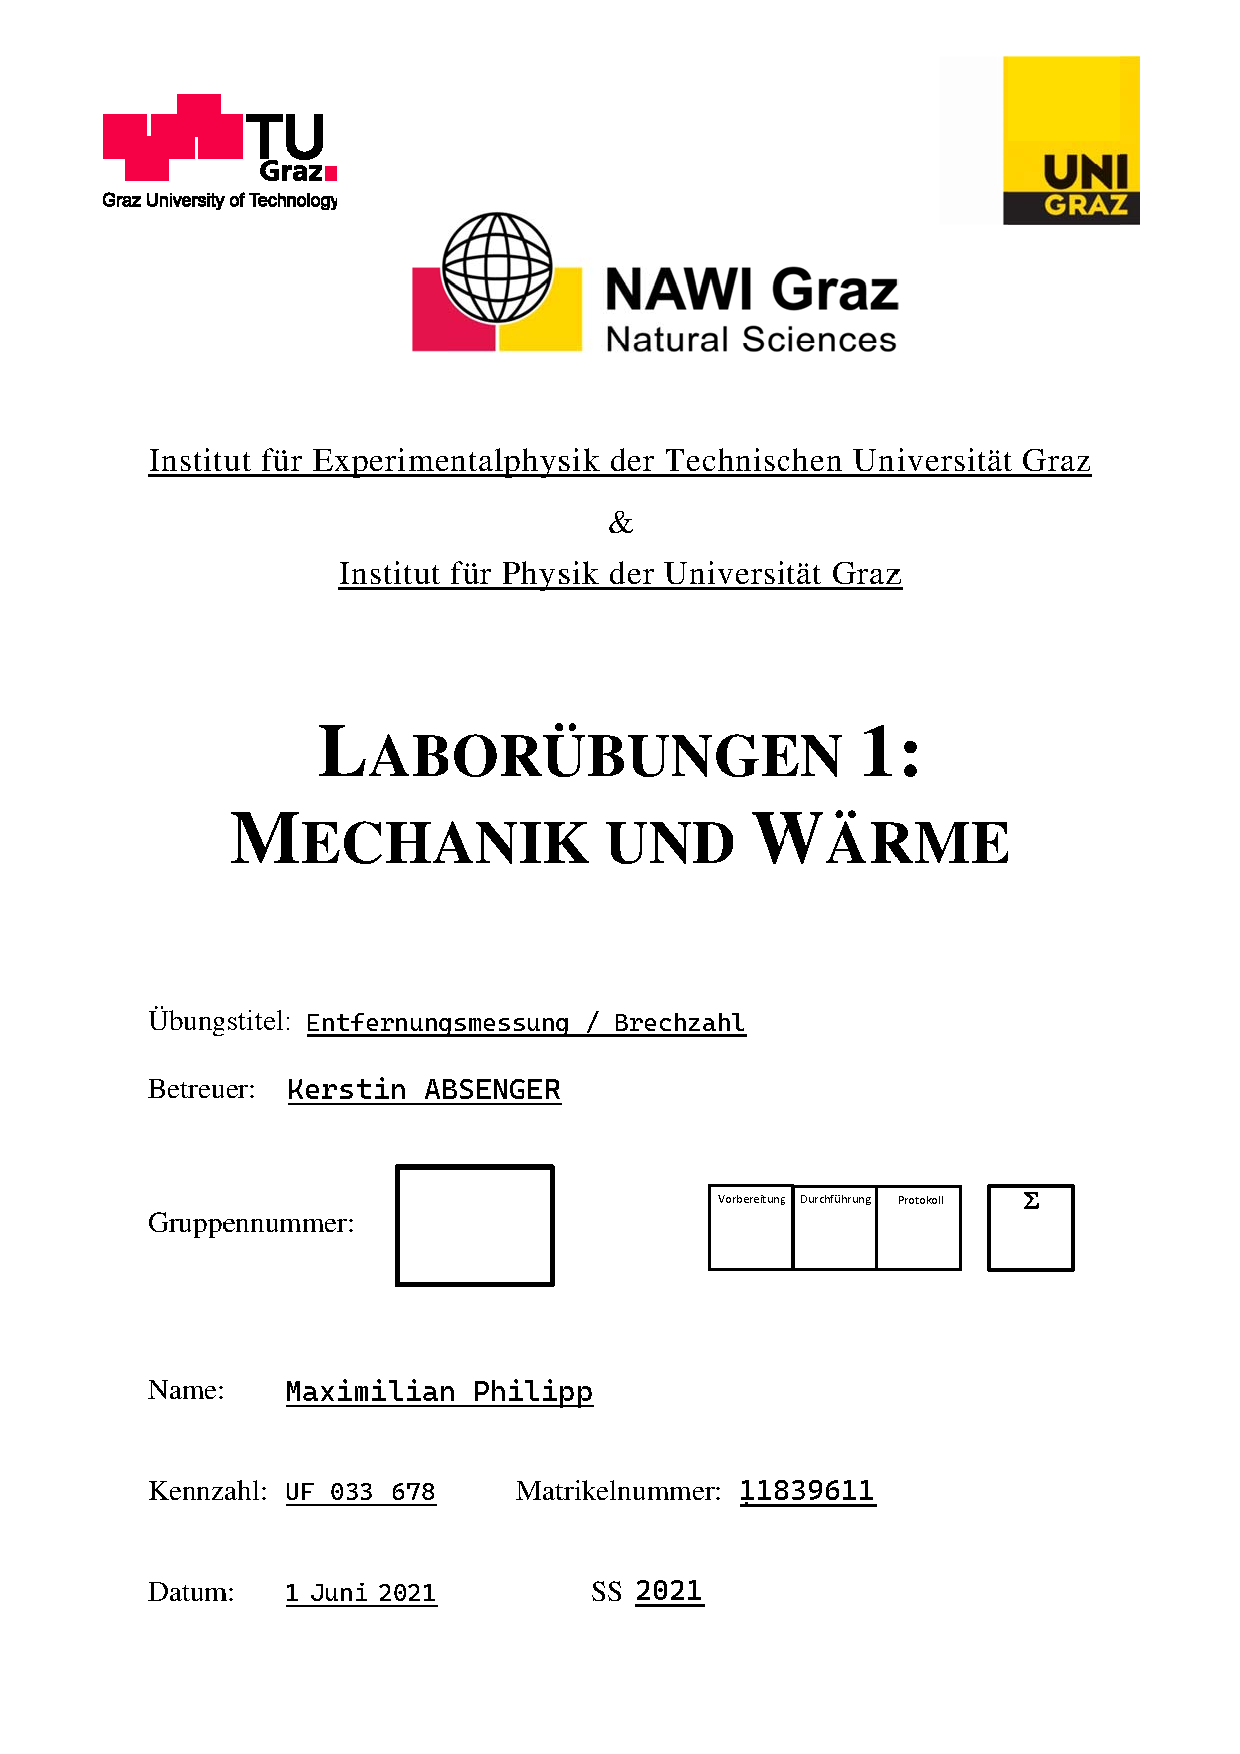
\includepdf{pdfs/Deckblatt.pdf} % Todo Deckblatt ausfüllen

\tableofcontents
\newpage
\section{Aufgabenstellung}
\label{sec:aufgabenstellung} 

\begin{enumerate}
    \item Zunächst die Herleitung der Formel $n = 1 + \frac{b-a}{a-h}$, mittels
        welcher, der Brechungsindex $n$ von einer unbekannten Flüssigkeit, mit
        dem Laser-Distanzmesser (LDM), bestimmt werden kann.  Die Variablen der
        Formel werden in \nameref{sec:voraussetzungen_grundlagen} genauer
        erklärt und im Kontext zu dem Experiment gebracht.  
    \item Messung der Brechzahlen von Wasser
        und 4 weiteren Flüssigkeiten mit dem Laserentfernungsmesser, unter Beachtung der Angaben aus dem
        Datenblatt des Entfernungsmessers. Die
        Brechzahl $n$ von Vakuum beträgt dabei 1 und von Luft 1,0003.  
    \item Erstellung einer Unsicherheitsanalyse der derart
        erhaltenen Brechzahlen, und Vergleich der so erhaltenen Brechzahlen
        mit jenen aus der Literatur.
\end{enumerate}

\section{Voraussetzungen und Grundlagen} \label{sec:voraussetzungen_grundlagen}
Folgende Grundlagen wurden aus dem zur Verfügung gestellten Vorlagenblatt
\cite{vorlageentfernung2021} und dem Mechanik Vorlesungskript \cite{Knoll2020}
entnommen und für dieses Experiment leicht angepasst.

Im Jahr 1983 wurde der Wert der Lichtgeschwindigkeit mit $c$ = 299 792 458 m/s
festgelegt. Auf der Definition und der Möglichkeit kurze Zeiten elektronisch zu
messen, beruhen die ``Laserpistole'' der Polizei und das ``elektronische Maßband'',
der Laser-Distanzmesser aus dem Baumarkt.

Die Funktion des Laser-Distanzmessers (LDM) ist eine elektronische Variante der
Zahnradmethode von Fizeau und im Prinzip einfach: Ein intensitätsmodulierter
Laserstrahl wird diffus an einem Objekt gestreut. Aus der Phasenverschiebung
der reflektierten Lichtpakete gegenüber den emittierten Paketen wird die
Laufzeit ermittelt, die mittels der Lichtgeschwindigkeit (in Luft) in
Entfernungen umgerechnet wird. Für Laien tritt ein überraschender Effekt auf,
wenn der Laserstrahl dabei ein transparentes Medium durchläuft. Die angezeigte
Distanz ist größer und daher „falsch“, das Licht hat länger gebraucht. Dies
legt nahe: Die Lichtgeschwindigkeit im Medium ist geringer als in Luft.

\begin{wrapfigure}{l}{0.4\textwidth}
        \centering
        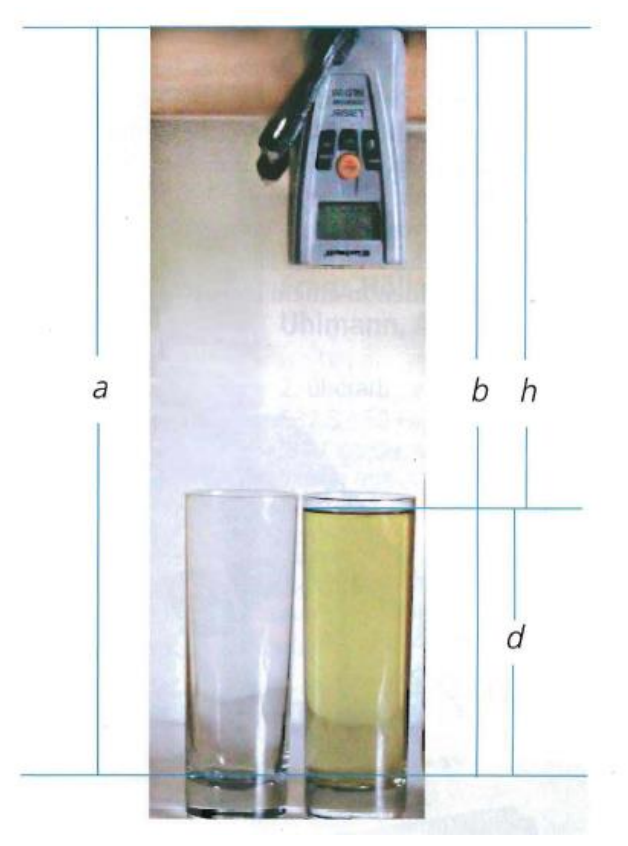
\includegraphics[width=0.9\linewidth]{pics/Messskizze.png}
        \caption{Messskizze}%
        \label{fig:Messskizze}
        \vspace{-2.5cm}
\end{wrapfigure}
\autoref{fig:Messskizze} zeigt die Anordnung des durchzuführenden Experiments. Unter einem LDM
befindet sich ein schlankes Trinkglas, auf dessen Boden eine Münze liegt. Die
Münze legt eine definierte Reflexionsebene fest. Bei leerem Glas wird der
Abstand $a$ der Münze vom LDM gemessen. Nachdem Wasser, Zuckerlösung, Glyzerin
oder eine andere transparente Flüssigkeit z.B. $d$ = 10 cm hoch eingefüllt wurde
- in der Abbildung ist zur besseren Sichtbarkeit Apfelsaft verwendet - wird der
Münzenabstand $b$ wieder gemessen. Als Wert ergibt sich $b > a$. Der optische Weg
ist also größer geworden. Schließlich lässt man auf der Flüssigkeitsoberfläche
ein kleines Stück Papier schwimmen, um die Entfernung $h$ des LDM von der
Oberfläche zu bestimmen. (Die Entfernungsangaben des LDM beziehen sich
üblicherweise auf die hintere Kante des Geräts.)


Da das LDM auf den Brechnungindex von Luft kalibriert ist, ist die gemessene
Laufzeit $T$ gleich dem gemessenen optischen Weg $b$ dividiert durch
die Lichtgeschwindigkeit in Luft $c_L$ also:

\begin{equation}
    T =  \frac{b}{c_L} \label{eq:laufzeit}
\end{equation}

Diese Zeit teilt sich in die Zeit $t_L$ auf, die das Licht benötigt, 
um Distanz $h$ in Luft zurückzulegen und in die Zeit $t_M$ die, das 
Licht benötigt, um Distanz $a-h$ im Medium zurückzulegen.

\begin{equation}
    T = t_L + t_M  = \frac{h}{c_L} + \frac{a-h}{c_M}  \label{eq:zeitaufteilung}
\end{equation}

Wobei $c_M$ die Lichtgeschwindigkeit im Medium ist.

Setzt man nun \autoref{eq:laufzeit} in \autoref{eq:zeitaufteilung}
ein und formt um, erhält man folgenden Ausdruck:

\begin{equation}
    \frac{b-h}{c_L} = \frac{a-h}{c_M} \label{eq:zeiten}
\end{equation}

Bringt man nun \autoref{eq:zeiten}, durch Umformungen, auf die Definition von
der Brechzahl $n=\frac{c_0}{c_M}$ erhält man:

\begin{equation}
    n = \frac{c_L}{c_M} = \frac{b-a+a-h}{a-h} = 1 + \frac{b-a}{a-h} \label{eq:brechzahl}
\end{equation}
Wobei angenommen wurde, dass die Lichtgeschwindigkeit im Vakuum $c_0$
gleich der Lichtgeschwindigkeit in Luft $c_L$ ist.


Um zu sehen, wie sich die Unsicherheit der Messungen bis in die Ergebnisse 
fortpflanzt, ist \autoref{eq:Unsicherheitsfortpflanzung} verwendet worden.
Die Grundlagen dieser Gleichung sind von den Powerpointfolien von 
GUM entnommen worden.\cite{WolfgangKessel2004} Die Verallgemeinerung stammt von Wikipedia
worden \cite{2020Fehler}.
Für die Auswertung ist die Progammiersprache Python im speziellen das 
Packet \verb#scipy#, zu Hilfe genommen worden.

\begin{equation}
    \label{eq:Unsicherheitsfortpflanzung}
    V_y = J(x) \cdot V_x \cdot J^{T}(x)
\end{equation}

Wobei $V_y$ und $V_x$ die Kovarianzmatrizen von den Vektoren $\bm{y}$ und $\bm{x}$ sind.
$\bm{x}$ ist der Vektor der Eingangsvariablen und $\bm{y}$ ist der Vektor der Ausgangsvariablen.
$J$ ist die Jakobimatrix der vektorwertigen Funktion $\bm{y} = \vec{F}(\bm{x})$ ist.
So lassen sich die Komponenten der Matrix relativ einfach anschreiben $J_{ij}(x) = \frac{\partial{y_i}}{\partial{x_j}}(x)$.
Damit man die Unsicherheit der einzelnen Variablen $y_i$ bekommt, muss nur die Quadratwurzel des i-ten Diagonalelements der 
$\bm{y}$-Kovarianzmatrix genommen werden $u_i= \sqrt{\mathrm{diag}(V_y)_i}$.
Da in diesem Experiment meistens nur skalare Funktionen untersucht werden, vereinfacht
sich die \autoref{eq:Unsicherheitsfortpflanzung} dramatisch und die Unsicherheit
der Variable $y$ lässt sich einfach so berechnen:

\begin{equation}
    \label{eq:graduncentainty}
    u_y = \sqrt{\mathrm{grad} y^T \cdot V_x \cdot \mathrm{grad} y}
\end{equation}

\section{Versuchsanordnung}
\label{sec:versuchsanordnung}

Es werden zwei Schragen gegenüber von einander gestellt und mit einem Brett
oben und einem Brett bei den Verstrebungen unten verbunden. Nun stellt man ein
Glas auf das untere Brett, wobei sich eine Münze am Boden des Gefäßes befindet,
siehe \autoref{fig:munze}.  Diese dient als definierte Reflexionsebene. Das
obere Brett dient als Referenzpunkt, damit immer die gleiche Distanz gemessen
wird. Weiters wurde das obere Brett beschwert, damit es sich beim Messen nicht
unabsichtlich hebt oder bewegt. Hier wurde die freihand Methode, verwendet.
Das heißt, dass der Laserentfernungsmesser nur beim Messen gegen die
Referenzfläche gehalten wird, siehe \autoref{fig:aufbau}.


\begin{figure}[H]
    \centering
    \begin{minipage}[htbp]{\linewidth}
        \begin{minipage}[htbp]{.45\linewidth} % [b] => Ausrichtung an \caption
            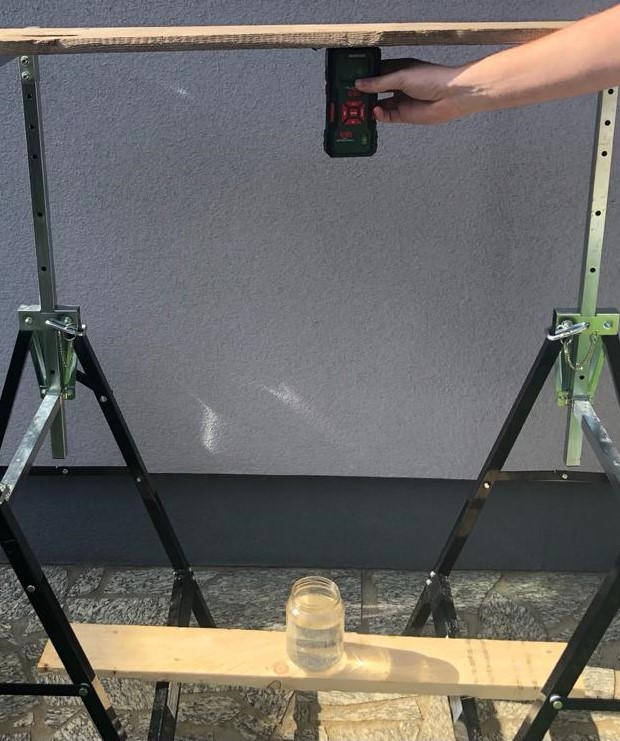
\includegraphics[width=\linewidth]{pics/aufbau1.jpeg}
        \caption[Aufbau des Experiments]{Aufbau des Experiments, wo ein Brett
            oben als Referenzfläche und ein Brett unten als Abstellfläche, zwischen
            die zwei Schragen gelegt werden.
        }
        \label{fig:aufbau}
        \end{minipage}
        \begin{minipage}[htbp]{.54\linewidth} % [b] => Ausrichtung an \caption
            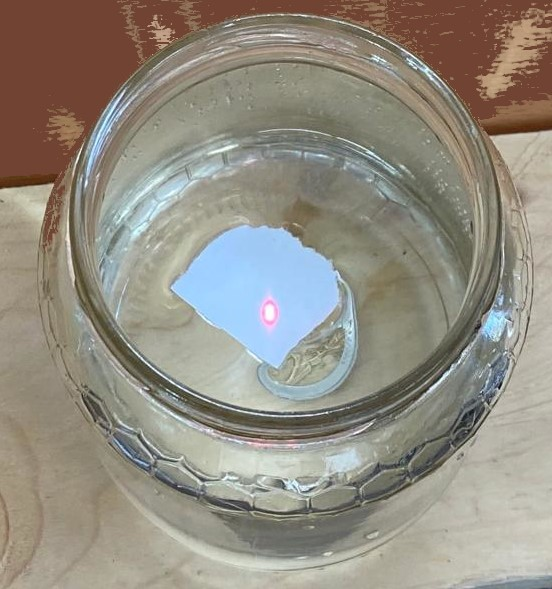
\includegraphics[width=\linewidth]{pics/aufbau2.jpeg}
        \caption[Aufbau der Reflexionsebene]{Aufbau der definierten Reflexionsebene 
        mit einer Münze im Gefäß}
        \label{fig:munze}
        \end{minipage}
    \end{minipage}
 \end{figure}


\section{Geräteliste}
\label{sec:geraeteliste}
%\setlength\LTleft{-6.5em}
\begin{longtable}{c|c|S|p{15em}}
\caption[Geräteliste]{Verwendete Geräte \label{tab:geraeteliste}} \\  % optionales Argument wird in Verzeichnissen verwendet, essentielles Argument direkt im Text
\toprule
Gerät                              & Gerät-Nr. & { Unsicherheit }  & Bemerkungen \\  
\midrule
\endfirsthead
\caption[]{(Fortsetzung)}\\
\toprule
Gerät                              & Gerät-Nr. & { Unsicherheit }  & Bemerkungen \\                                                                        
\midrule
\endhead
\endfoot
\endlastfoot
        Brett, lang            & axx & { - }       & Dient als Referenzpunkt für die Distanzmessungen\\ \hline
        Laserentfernungsmesser & bxx & \SI{5}{\mm} & Um die Laufzeit in verschiedener Medien indirekt zu messen. Messbereich: \SIrange{0.175}{20}{\meter} \cite{laserdistanzmesser}\\ \hline
        Joghurt Glas           & cxx & { - }       & Ein Gefäß um die Flüssigkeiten zu halten\\ \hline
        Brett, kurz            & dxx & { - }       & Dient als Oberfläche um das Glas drauf zu stellen\\ \hline
        Schragen 2x            & fxx & { - }       & Dient als Lager für die Bretter \\ \hline
        Gewichte               & gxx & { - }       & Um das obere Brett zu fixieren\\ \hline
        Wasser, kalkhaltig     & hxx & { - }       & Erstes Medium von dem der Brechungsindex bestimmt wird.\\ \hline
        Rapsöl                     & ixx & { - }       & Zweites Medium von dem der Brechungsindex bestimmt wird.\\ \hline
        Holundersaft pur      & jxx & { - }       & Drittes Medium von dem der Brechungsindex bestimmt wird.\\ \hline
        Minearalwasser        & kxx & { - }       & Viertes Medium von dem der Brechungsindex bestimmt wird.\\ \hline
        Ethanol \SI{96}{\percent} & lxx & { - } & Fünftes Medium von dem der Brechungsindex bestimmt wird.\\ \hline

        \hline
\end{longtable}

\section{Versuchsdurchführung und Messergebnisse}
\label{sec:versuchsdurchfuehrung_messergebnisse}
Im folgenden Ablauf wird beschrieben, wie der Aufbau nach 
dem Kapitel \nameref{sec:versuchsanordnung} verwendet wird
um die gesuchten Werte zu erhalten. Damit nach \autoref{eq:brechzahl}
die Brechzahl diverser Flüssigkeiten bestimmt werden kann.

\subsection{Ablauf}
\begin{enumerate} \label{en:Ablauf}
    \item Falls das Gefäß befüllt ist, muss das Gefäß entleert, gereinigt und getrocknet werden.
    \item Nun füllt man die neue Flüssigkeit in das Gefäß und stellt es auf das untere Brett.
    \item Man nimmt das Laser-Distanzmessgerät und hält es gegen die Referenzebene. Weiters schaut
        man, dass sich das Gerät über dem Gefäß befindet und der Laserpunkt auf der Münze ist.
    \item Nun wird der gemessene Wert für die Distanz $b$ notiert.
    \item Nach der Messung wird ein Stück Papier auf die Oberfläche der Flüssigkeit gelegt, sodass
        dieses Stück nicht untergeht.
    \item Nun wird wieder das Laser-Distanzmessgerät verwendet um die Distanz $h$ vom Brett
        zur Oberfläche der Flüssigkeit zu messen. Diese Distanz wird wieder notiert.
    \item Dieser Prozess wird für alle Flüssigkeiten wiederholt.
\end{enumerate}

Durch Durchführen dieses Ablaufs, erhält man folgende Werte für die diversen Flüssigkeiten:

\begin{table}[H]
    \centering
    \caption{
        Diese Tabelle beinhaltet die, von dem LDM gemessenen, Distanzen die
        durch Durchführen dieses \hyperref[en:Ablauf]{Ablaufs} gefunden werden.\\ 
        $b$ ist der gemessene Abstand von der Münze zum oberen Brett $\Delta b=\SI{5}{\mm}$ \\
        $h$ ist der gemessene Abstand von der Oberfläche zum oberen Brett $\Delta h = \SI{5}{\mm}$\\
    }
    \label{tab:messwerte_distanzen}
    \begin{tabular}{l|S|S|S|S}
        Flüssigkeit        & {$b$}        & {$h$}        \\ \hline
        {}                 & {/ \si{\mm}} & {/ \si{\mm}} \\ \hline \hline
        Wasser, kalkhaltig & 1025         & 899          \\
        Rapsöl             & 1041         & 901          \\
        Holundersaft pur   & 1039         & 905          \\
        Minearalwasser    & 1022         & 913          \\
        Ethanol \SI{96}{\percent} & 1028         & 910          \\
    \end{tabular}
\end{table}

Dabei ist zu erwähnen, dass die Messwerte der Längen die Länge des Geräts inkludieren.

Weiters wurde auch die Distanz $a$ von der Münze bis zum oberen Brett ohne, dass das Glas
mit einer Flüssigkeit befüllt ist bestimmt. Indem der oberen \hyperref[en:Ablauf]{Ablauf}
ohne Befüllen des Glases ausgeführt wird, bekommt man folgenden Wert:

\begin{equation}
    a = \SI{998(5)}{\mm}
\end{equation}



\section{Auswertung}
\label{sec:auswertung}

Kombiniert man die Werte aus \autoref{tab:messwerte_distanzen} und dem Wert für die
eigentliche Distanz $a$ zwischen dem Brett und der Münze mit
\autoref{eq:brechzahl}, erhält man folgende Werte für die Brechungsindexe $n$ für die
diversen Flüssigkeiten:


\begin{table}[H]
    \centering
    \caption{Diese Tabelle beinhaltet die erhaltenen Werte für
        die Brechzahlen diverser Flüssigkeiten. \\
    $n$ die Brechzahl der diversen Flüssigkeiten \\
}
    \label{tab:ausgewertet}
    \begin{tabular}{c|S|S}
        Flüssigkeit          & {$n$} & {$\Delta n$} \\ \hline
        Wasser, kalkhaltig   & 1.27  & 0.08         \\
        Rapsöl               & 1.44  & 0.09         \\
        Holundersaft pur     & 1.44  & 0.10         \\
        Minearalwasser      & 1.28  & 0.10         \\
        Ethanol \SI{96}{\percent}      & 1.34  & 0.10         \\
    \end{tabular}
\end{table}

\section{Diskussion und Zusammenfassung}
\label{sec:diskussion_zusammenfassung}
% Aufzählung was scheiße glaufen is

Nun werden die verwendeten Methoden diskutiert und die Ergebnisse 
zusammengefasst.

\subsection{Diskussion}
Die erhaltenen Werte aus dem Kapitel \nameref{sec:auswertung} 
für die Brechungsindexe der diversen Flüssigkeiten wurden
in \autoref{tab:ergebnisse} den Literaturwerten gegenübergestellt.
Jedoch konnte leider kein Literaturwert für kaboniertes Wasser 
gefunden werden, da dieser sich höchstwahrscheinlich nicht wirklich von
dem von Wasser unterscheidet.

\begin{table}[H]
    \centering
    \caption{Messergebnisse der Brechzahlen der diversen Flüssigkeiten und Vergleich mit den Literaturwerten.\\
    $n$ die Brechzahl einer Flüssigkeit}
    \label{tab:ergebnisse}
    \begin{tabular}{c|S|S|S}
        Flüssigkeit          & {$n$} & {$\Delta n$} & {Literaturwert}                         \\ \hline
        Wasser, kalkhaltig   & 1.27  & 0.08         & 1.33251 \cite{brechzahlwasser} \\
        Rapsöl               & 1.44  & 0.09         & \numrange{1.470}{1.474} \cite{brechzahloele}  \\
        Holundersaft pur     & 1.44  & 0.10         & \numrange{1.45}{1.46} \cite{brechzahlsirup} \\
        Minearalwasser      & 1.28  & 0.10         & { - } \\
        Ethanol \SI{96}{\percent}      & 1.34  & 0.10         & 1.3638 \cite{brechzahlethanol} \\
    \end{tabular}
\end{table}

Zwar beinhalten alle Werte die Literaturwerte in ihren Unsicherheitsintervallen,
jedoch liegen die Werte alle unter den Literaturwerten. Dies ist ein Indiz dafür, dass 
hier ein sytematischer Fehler vorliegt. Es könnte irgendwas im Messgerät (zb. eine Fehlkalibrierung, welche unterschiedliche Effekte bei
verschiedenen Distanzen hat) sein. Dies kann aber auch einfach nur ein Zufall
sein, was bei den großen Unsicherheitsintervallen der Längenmessungen 
durchaus der Fall sein kann. 

\subsection{Verbesserungsvorschläge}
\begin{enumerate}
    \item Ein genaueres Laser-Distanzmessgerät
    \item Über weitere Distanzen messen damit der relative Fehler kleiner wird
    \item Verwendung von einem flachen polierten Metallplättchen damit Streulicht minimiert wird.
    \item Eine stärkere und gerichtete Laserdiode verwenden, damit auch bei größeren Distanzen der
        Strahl noch immer ein starkes Signal gibt.
\end{enumerate}

\subsection{Zusammenfassung}
Da das vorhandene Laser-Distanzmessgerät leider nicht sehr genau
war, konnten auch keine genauen Werte für die Brechzahlen der 
diversen Flüssigkeiten bestimmt werden. Fehler durch Messen mit schlechten
Messgeräten nennt man im Fachjargon auch GIGO (``garbage in, garbage out'').
Was hier eindeutig vorliegt. Bestenfalls lässt sich sagen, dass sich mit den,
in diesem Experiment zur Verfügung gestandenen Mitteln, der Brechungsindex 
von Flüssigkeiten maximal auf eine Nachkommastelle genau bestimmen lässt.

Schlussendlich lässt sich sagen, dass in diesem Experiment der mangelnde Faktor
das Messgerät war, und beim nächsten Durchführen ein Genaueres verwendet werden soll.

% Literaturtabelle
\newpage
\printbibliography

\listoffigures

\listoftables


\end{document}
